\documentclass[../main.tex]{subfiles}

\begin{document}

\chapter{入门}

\section{示例}

正文在这里

\textbf{粗体}

\uline{下划线}


SRCNN~\cite{dong2014learning}, ESRGAN~\cite{wang2018esrgan}

BasicSR代码库解读(一): 使用场景和目录

拖延了一年的坑,今天开始来慢慢填了......  (基于BasicSR V1.3.4.2介绍)。

两种使用场景
BasicSR近期又更新了一波,主要支持两种使用场景。
一是 直接使用BasicSR的本地克隆仓库。我们可以方便地看到BasicSR的完整代码,修改并使用。例如,在BasicSR中训练SRGAN或者StyleGAN2。这种场景对应着通过从local clone中安装,即先git clone,再python setup.py develop/install。更多参考:\url{https://github.com/xinntao/BasicSR/blob/master/INSTALL.md#install-from-a-local-clone}二是 把BasicSR当作一个额外的python package - basicsr,即可以通过pip安装。它提供了训练的框架,流程和一些基本功能。你可以基于basicsr方便地搭建你自己的项目基。例如,基于basicsr搭建的Real-ESRGAN和基于basicsr搭建的GFPGAN。

大部分的深度学习项目,都可以分为以下几个部分:
● data: 定义了训练数据,来喂给模型的训练
● arch (architecture): 定义了网络结构和forward的步骤
● model: 定义了在训练中必要的组件(比如 loss) 和 一次完整的训练过程(包括前向传播,反向传播,梯度优化等),还有其他功能,比如validation等
● training pipeline: 定义了训练的流程,即把数据 dataloader,模型,validation,保存 checkpoints 等等串联起来
当我们开发一个新的方法时,我们往往在改进: data, arch, model;而很多流程、基础的功能其实是共用的。那么,我们希望可以专注于主要功能的开发,而不要重复造轮子。
因此便有了 BasicSR,它把很多相似的功能都独立出来,我们只要关心 data, arch, model 的开发即可。
为了进一步方便大家使用,我们提供了 basicsr package,大家可以通过  pip install basicsr 方便地安装,然后就可以使用 BasicSR 的训练流程以及在 BasicSR 里面已开发好的功能啦~
基于 basicsr package的使用指南
关于如何基于 basicsr 这个packag开发你自己的项目,我专门写了一个详细的指南,放在仓库BasicSR-example (https://github.com/xinntao/BasicSR-examples)里面了,大家可以参考那里呐~
BasicSR原仓库目录
本专栏主要讲解BasicSR原仓库的代码,对应着通过从local clone中安装,即先git clone,再python setup.py develop/install。
“看书看目录”。我们首先也来看一下BasicSR仓库的目录,先来整体地把握一下~ 其中红色的表示和跑实验直接相关的文件。


进一步的看,
basicsr文件夹中进一步有:(其中标红的表示我们开发中主要修改的文件)


scripts 文件夹中进一步有

至此,我们对BasicSR的整体框架便有了一定的了解啦~



\dirtree{%
	.1 /.
	.2 bin.
	.2 home.
	.3 jeancome.
	.4 texmf.
	.5 tex.
	.3 jeancomeson\DTcomment{注释}.
	.3 jeancomedaughter\DTcomment{这是说明啦}.
	.2 usr.
	.3 bin.
}


%\setlength{\columnsep}{0.7cm}
\begin{wrapfigure}{r}{0.4\linewidth}
%\vspace{-0.3cm}
\centering
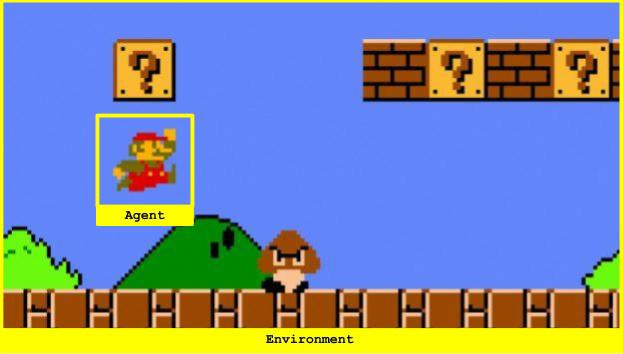
\includegraphics[width=0.4\textwidth]{figures/agentenv.png}
%\caption{Пример среды с двумя действиями.}
%\label{fig:env}
%\vspace{-2.6cm}
\end{wrapfigure}


\end{document}